\subsection{Impedance Simulations and Results}
\label{sec:imp-sims-tctp}

The impedance of the TCTP collimator is examined through the use of simulation codes. In order to verify the simulation results it was decided to use both a time domain and a frequency domain code, in this case CST Particle Studio for the time domain and Ansoft HFSS for the frequency domain. Due to the reduced simulation time for time domain simulations compared to frequency domain simulations (which must be evaluated mode by mode to correctly evaluate the eigenmodes), the preliminary comparisons are done using the time domain code and the most promising solutions are subsequently investigated in depth using the frequency domain model.

For this comparison we investigate a number of different designs of the RF system for comparison to the ferrite damping solution chosen for construction;

\begin{enumerate}
\item{The phase 1 sliding RF contacts. Shown in Fig.~\ref{fig:phase-1-rf}.}
\item{The proposed RF system including the ferrite damping tiles and the RF screen as shown in Fig.~\ref{fig:phase-2-rf-system}.}
\item{The proposed RF system without the ferrite damping tiles. This is too investigate the benefit of including the ferrite tiles.}
\end{enumerate}


\begin{figure}
\begin{center}
\subfigure[]{
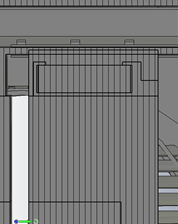
\includegraphics[width=0.3\textwidth]{LHC_Collimation_Upgrades/figures/tctp-closed.png}
\label{fig:sliding-contacts}
}
\subfigure[]{
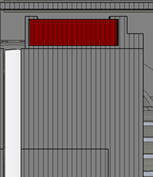
\includegraphics[width=0.3\textwidth]{LHC_Collimation_Upgrades/figures/tctp-ferrite.png}
\label{fig:rf-circuit-ferrite}
}
\end{center}
\caption{The different RF systems considered for the TCTP collimator. \ref{fig:sliding-contacts} shows an RF system similar to the phase 1 RF system. In these simulations the sliding RF contacts are replaced by a perfect connection - for frequencies lower than 2-3GHz this is a good approximation and greatly simplifies the simulation model. \ref{fig:rf-circuit-ferrite} shows the RF circuit complete with ferrite. Two further variants may be considered, where the ferrite is replaced by either vacuum (to indentify how the ferrite damps the otherwise present modes) and replacing the ferrite with PEC (to see whether it is the ferrite or the small aperture that reduces the coupling of the beam to the surrounding vacuum tank).}
\label{fig:rf-systems-tctp}
\end{figure}


The three different systems are shown in Fig.~\ref{fig:rf-systems-tctp}. The impedance results for these three options are shown in Fig.~\ref{fig:tctp-time-longitudinal} simulated in CST Particle Studio. It can clearly be seen the differences between the two RF systems. The phase 1 RF system screens the surrounding vacuum tank from the beam, meaning any cavity modes occur at a relatively high frequency, above 1GHz. The phase 2 system allows the beam to see the vacuum cavity, decreasing the lowest frequency cavity mode. The presence of the ferrite in this system subsequently strongly reduces the Q of these resonances, reducing the impedance. Both the real and imaginary longitudinal impedance is strongly reduced as a result. Similar results have been observed in the transverse plane \cite{Salvant:tctp}.

\begin{figure}
\begin{center}
\subfigure[]{
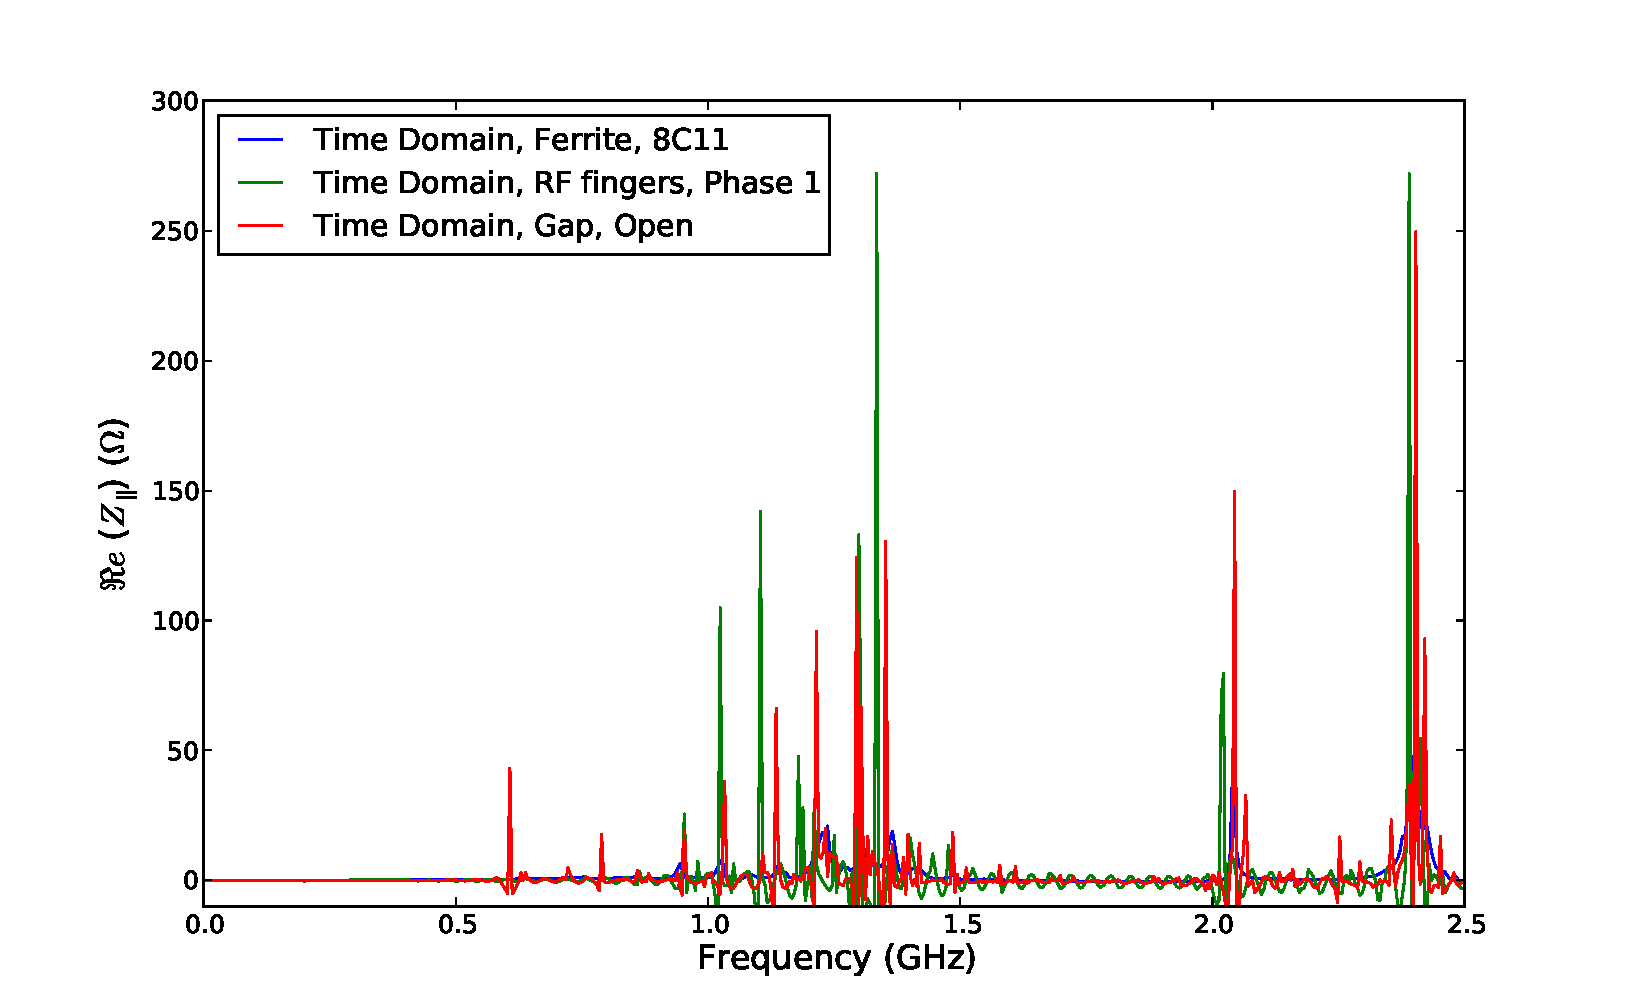
\includegraphics[width=0.7\textwidth]{LHC_Collimation_Upgrades/figures/impedance-tctp-time.pdf}
\label{fig:tctp-time-real}
}

\subfigure[]{
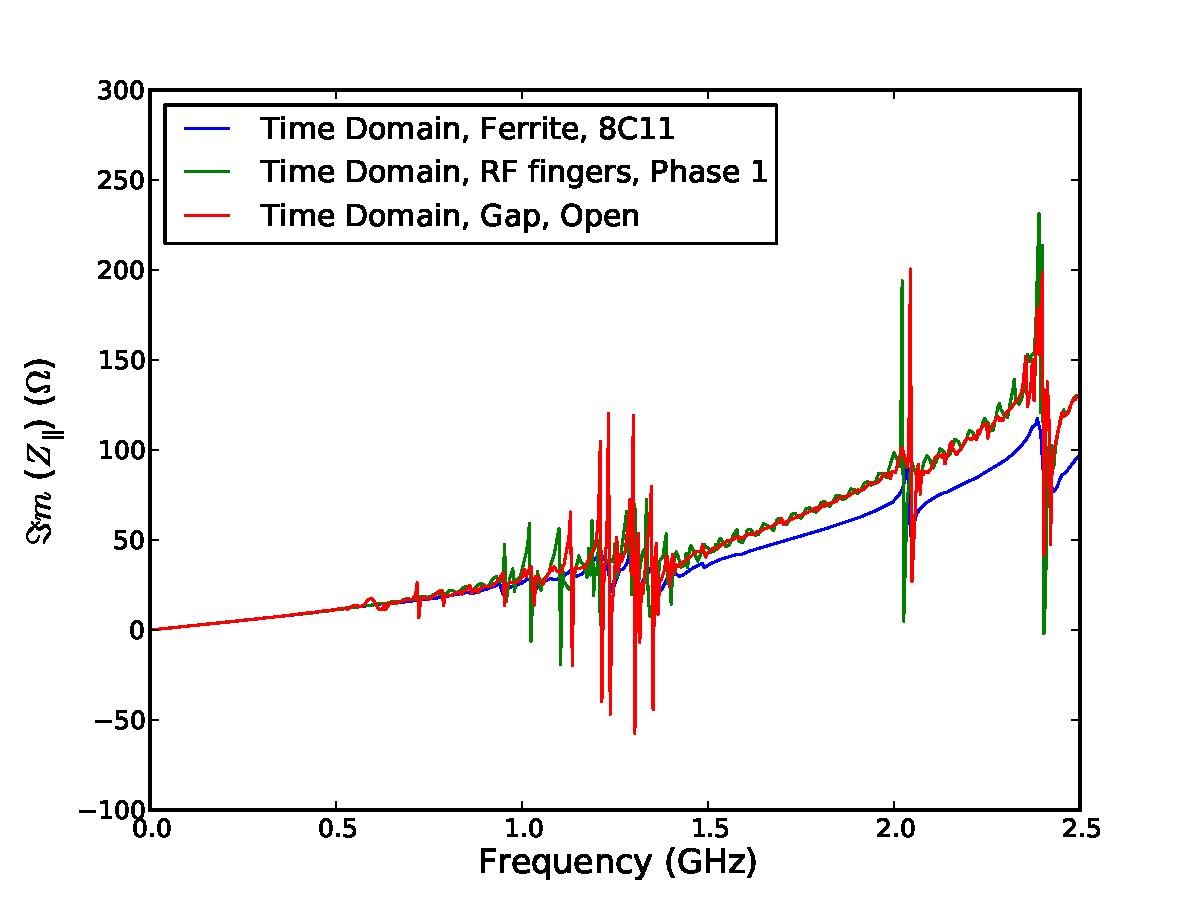
\includegraphics[width=0.7\textwidth]{LHC_Collimation_Upgrades/figures/impedance-tctp-time-imag.pdf}
\label{fig:tctp-time-imag}
}
\end{center}
\caption{The longitudinal impedance of the TCTP collimator for a number different configurations. Shown is the system using the ferrite damping system (ferrite being 8C11 in this case), RF fingers as in phase 1, and the RF system with the ferrite replaced by PEC. The real \ref{fig:tctp-time-real} and imaginary \ref{fig:tctp-time-imag} components are shown.}
\label{fig:tctp-time-longitudinal}
\end{figure}


